\begin{exercice}
    \begin{minipage}{0.5\linewidth}
        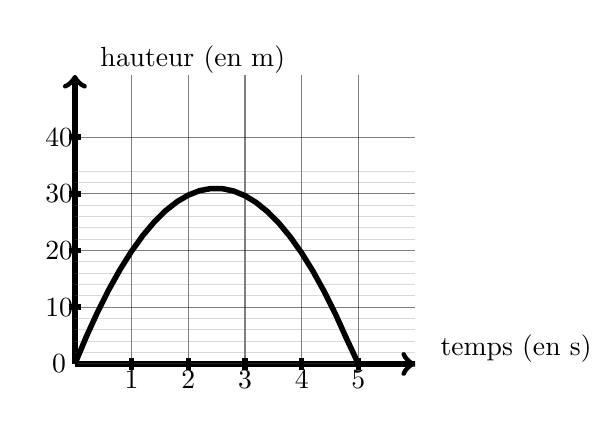
\begin{tikzpicture}[baseline,scale=0.4]

            \tikzset{
            point/.style={
                thick,
                draw,
                cross out,
                inner sep=0pt,
                minimum width=5pt,
                minimum height=5pt,
            },
            }
            \clip (-1.5,-1.5) rectangle (16.3,10.675571413994916);


                
            \draw[color ={black},line width = 2,->] (0,0)--(10.8,0);
            \draw[color ={black},line width = 2,->] (0,0)--(0,9.175571413994916);
            \draw[color ={black},opacity = 0.5] (0,1.8000000000000003)--(10.8,1.8000000000000003);
            \draw[color ={black},opacity = 0.5] (0,3.6000000000000005)--(10.8,3.6000000000000005);
            \draw[color ={black},opacity = 0.5] (0,5.4)--(10.8,5.4);
            \draw[color ={black},opacity = 0.5] (0,7.200000000000001)--(10.8,7.200000000000001);
            \draw[color ={black},opacity = 0.5] (1.8,0)--(1.8,9.175571413994916);
            \draw[color ={black},opacity = 0.5] (3.6,0)--(3.6,9.175571413994916);
            \draw[color ={black},opacity = 0.5] (5.4,0)--(5.4,9.175571413994916);
            \draw[color ={black},opacity = 0.5] (7.2,0)--(7.2,9.175571413994916);
            \draw[color ={black},opacity = 0.5] (9,0)--(9,9.175571413994916);
            \draw[color ={gray},opacity = 0.3] (0,0)--(10.8,0);
            \draw[color ={gray},opacity = 0.3] (0,0.36000000000000004)--(10.8,0.36000000000000004);
            \draw[color ={gray},opacity = 0.3] (0,0.7200000000000001)--(10.8,0.7200000000000001);
            \draw[color ={gray},opacity = 0.3] (0,1.08)--(10.8,1.08);
            \draw[color ={gray},opacity = 0.3] (0,1.4400000000000002)--(10.8,1.4400000000000002);
            \draw[color ={gray},opacity = 0.3] (0,2.16)--(10.8,2.16);
            \draw[color ={gray},opacity = 0.3] (0,2.5200000000000005)--(10.8,2.5200000000000005);
            \draw[color ={gray},opacity = 0.3] (0,2.8800000000000003)--(10.8,2.8800000000000003);
            \draw[color ={gray},opacity = 0.3] (0,3.24)--(10.8,3.24);
            \draw[color ={gray},opacity = 0.3] (0,3.9600000000000004)--(10.8,3.9600000000000004);
            \draw[color ={gray},opacity = 0.3] (0,4.32)--(10.8,4.32);
            \draw[color ={gray},opacity = 0.3] (0,4.680000000000001)--(10.8,4.680000000000001);
            \draw[color ={gray},opacity = 0.3] (0,5.040000000000001)--(10.8,5.040000000000001);
            \draw[color ={gray},opacity = 0.3] (0,5.760000000000001)--(10.8,5.760000000000001);
            \draw[color ={gray},opacity = 0.3] (0,6.120000000000001)--(10.8,6.120000000000001);
            \draw[color ={black},line width = 2] (1.8,-0.2)--(1.8,0.2);
            \draw[color ={black},line width = 2] (3.6,-0.2)--(3.6,0.2);
            \draw[color ={black},line width = 2] (5.4,-0.2)--(5.4,0.2);
            \draw[color ={black},line width = 2] (7.2,-0.2)--(7.2,0.2);
            \draw[color ={black},line width = 2] (9,-0.2)--(9,0.2);
            \draw[color ={black},line width = 2] (-0.2,1.8000000000000003)--(0.2,1.8000000000000003);
            \draw[color ={black},line width = 2] (-0.2,3.6000000000000005)--(0.2,3.6000000000000005);
            \draw[color ={black},line width = 2] (-0.2,5.4)--(0.2,5.4);
            \draw[color ={black},line width = 2] (-0.2,7.200000000000001)--(0.2,7.200000000000001);
            \draw [color={black},fill opacity = 1] (1.8,-0.5) node[anchor = center,scale=1] {$1$};
            \draw [color={black},fill opacity = 1] (3.6,-0.5) node[anchor = center,scale=1] {$2$};
            \draw [color={black},fill opacity = 1] (5.4,-0.5) node[anchor = center,scale=1] {$3$};
            \draw [color={black},fill opacity = 1] (7.2,-0.5) node[anchor = center,scale=1] {$4$};
            \draw [color={black},fill opacity = 1] (9,-0.5) node[anchor = center,scale=1] {$5$};
            \draw [color={black},fill opacity = 1] (-0.5,1.8000000000000003) node[anchor = center,scale=1] {$10$};
            \draw [color={black},fill opacity = 1] (-0.5,3.6000000000000005) node[anchor = center,scale=1] {$20$};
            \draw [color={black},fill opacity = 1] (-0.5,5.4) node[anchor = center,scale=1] {$30$};
            \draw [color={black},fill opacity = 1] (-0.5,7.200000000000001) node[anchor = center,scale=1] {$40$};
            \draw [color={black},fill opacity = 1] (11.3,0.5) node[anchor = west,scale=1] {temps (en s)};
            \draw [color={black},fill opacity = 1] (0.5,9.675571413994916) node[anchor = west,scale=1] {hauteur (en m)};
            
            \draw[color={black},line width = 2] (0,0)--(0.36000000000000004,0.8600457131195933)--(0.7200000000000001,1.6480914262391866)--(1.0800000000000003,2.36413713935878)--(1.4400000000000002,3.0081828524783734)--(1.8,3.580228565597966)--(2.16,4.080274278717559)--(2.52,4.508319991837152)--(2.88,4.864365704956746)--(3.2399999999999998,5.148411418076339)--(3.5999999999999996,5.360457131195932)--(3.9599999999999995,5.500502844315525)--(4.32,5.568548557435119)--(4.680000000000001,5.564594270554711)--(5.040000000000001,5.488639983674304)--(5.400000000000001,5.340685696793898)--(5.760000000000002,5.120731409913492)--(6.120000000000002,4.828777123033084)--(6.480000000000002,4.4648228361526785)--(6.8400000000000025,4.028868549272267)--(7.200000000000002,3.5209142623918637)--(7.560000000000002,2.9409599755114524)--(7.920000000000003,2.289005688631045)--(8.280000000000003,1.565051401750637)--(8.640000000000002,0.7690971148702276)--(9.000000000000004,0)--(9.360000000000003,0)--(9.720000000000004,0)--(10.080000000000004,0)--(10.440000000000005,0)--(10.800000000000004,0);
            \draw [color={black},fill opacity = 1] (-0.5,0) node[anchor = center,scale=1] {$0$};

        \end{tikzpicture}
    \end{minipage}
    \begin{minipage}{0.43\linewidth}
        On a représenté l'évolution de la hauteur d'un projectile lancé depuis le sol (en m) en fonction du temps (en secondes).    
        \begin{enumerate}
            \item Déterminer au bout de combien de temps le projectile retombe au sol.
            \item Déterminer la hauteur maximale atteinte par le projectile.
        \end{enumerate}
    \end{minipage}
\end{exercice}
\begin{corrige}
        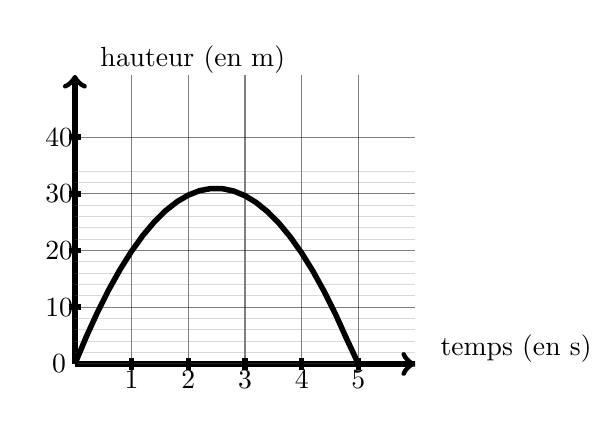
\begin{tikzpicture}[baseline,scale=0.4]

            \tikzset{
            point/.style={
                thick,
                draw,
                cross out,
                inner sep=0pt,
                minimum width=5pt,
                minimum height=5pt,
            },
            }
            \clip (-1.5,-1.5) rectangle (16.3,10.675571413994916);


                
            \draw[color ={black},line width = 2,->] (0,0)--(10.8,0);
            \draw[color ={black},line width = 2,->] (0,0)--(0,9.175571413994916);
            \draw[color ={black},opacity = 0.5] (0,1.8000000000000003)--(10.8,1.8000000000000003);
            \draw[color ={black},opacity = 0.5] (0,3.6000000000000005)--(10.8,3.6000000000000005);
            \draw[color ={black},opacity = 0.5] (0,5.4)--(10.8,5.4);
            \draw[color ={black},opacity = 0.5] (0,7.200000000000001)--(10.8,7.200000000000001);
            \draw[color ={black},opacity = 0.5] (1.8,0)--(1.8,9.175571413994916);
            \draw[color ={black},opacity = 0.5] (3.6,0)--(3.6,9.175571413994916);
            \draw[color ={black},opacity = 0.5] (5.4,0)--(5.4,9.175571413994916);
            \draw[color ={black},opacity = 0.5] (7.2,0)--(7.2,9.175571413994916);
            \draw[color ={black},opacity = 0.5] (9,0)--(9,9.175571413994916);
            \draw[color ={gray},opacity = 0.3] (0,0)--(10.8,0);
            \draw[color ={gray},opacity = 0.3] (0,0.36000000000000004)--(10.8,0.36000000000000004);
            \draw[color ={gray},opacity = 0.3] (0,0.7200000000000001)--(10.8,0.7200000000000001);
            \draw[color ={gray},opacity = 0.3] (0,1.08)--(10.8,1.08);
            \draw[color ={gray},opacity = 0.3] (0,1.4400000000000002)--(10.8,1.4400000000000002);
            \draw[color ={gray},opacity = 0.3] (0,2.16)--(10.8,2.16);
            \draw[color ={gray},opacity = 0.3] (0,2.5200000000000005)--(10.8,2.5200000000000005);
            \draw[color ={gray},opacity = 0.3] (0,2.8800000000000003)--(10.8,2.8800000000000003);
            \draw[color ={gray},opacity = 0.3] (0,3.24)--(10.8,3.24);
            \draw[color ={gray},opacity = 0.3] (0,3.9600000000000004)--(10.8,3.9600000000000004);
            \draw[color ={gray},opacity = 0.3] (0,4.32)--(10.8,4.32);
            \draw[color ={gray},opacity = 0.3] (0,4.680000000000001)--(10.8,4.680000000000001);
            \draw[color ={gray},opacity = 0.3] (0,5.040000000000001)--(10.8,5.040000000000001);
            \draw[color ={gray},opacity = 0.3] (0,5.760000000000001)--(10.8,5.760000000000001);
            \draw[color ={gray},opacity = 0.3] (0,6.120000000000001)--(10.8,6.120000000000001);
            \draw[color ={black},line width = 2] (1.8,-0.2)--(1.8,0.2);
            \draw[color ={black},line width = 2] (3.6,-0.2)--(3.6,0.2);
            \draw[color ={black},line width = 2] (5.4,-0.2)--(5.4,0.2);
            \draw[color ={black},line width = 2] (7.2,-0.2)--(7.2,0.2);
            \draw[color ={black},line width = 2] (9,-0.2)--(9,0.2);
            \draw[color ={black},line width = 2] (-0.2,1.8000000000000003)--(0.2,1.8000000000000003);
            \draw[color ={black},line width = 2] (-0.2,3.6000000000000005)--(0.2,3.6000000000000005);
            \draw[color ={black},line width = 2] (-0.2,5.4)--(0.2,5.4);
            \draw[color ={black},line width = 2] (-0.2,7.200000000000001)--(0.2,7.200000000000001);
            \draw [color={black},fill opacity = 1] (1.8,-0.5) node[anchor = center,scale=1] {$1$};
            \draw [color={black},fill opacity = 1] (3.6,-0.5) node[anchor = center,scale=1] {$2$};
            \draw [color={black},fill opacity = 1] (5.4,-0.5) node[anchor = center,scale=1] {$3$};
            \draw [color={black},fill opacity = 1] (7.2,-0.5) node[anchor = center,scale=1] {$4$};
            \draw [color={black},fill opacity = 1] (9,-0.5) node[anchor = center,scale=1] {$5$};
            \draw [color={black},fill opacity = 1] (-0.5,1.8000000000000003) node[anchor = center,scale=1] {$10$};
            \draw [color={black},fill opacity = 1] (-0.5,3.6000000000000005) node[anchor = center,scale=1] {$20$};
            \draw [color={black},fill opacity = 1] (-0.5,5.4) node[anchor = center,scale=1] {$30$};
            \draw [color={black},fill opacity = 1] (-0.5,7.200000000000001) node[anchor = center,scale=1] {$40$};
            \draw [color={black},fill opacity = 1] (11.3,0.5) node[anchor = west,scale=1] {temps (en s)};
            \draw [color={black},fill opacity = 1] (0.5,9.675571413994916) node[anchor = west,scale=1] {hauteur (en m)};
            
            \draw[color={black},line width = 2] (0,0)--(0.36000000000000004,0.8600457131195933)--(0.7200000000000001,1.6480914262391866)--(1.0800000000000003,2.36413713935878)--(1.4400000000000002,3.0081828524783734)--(1.8,3.580228565597966)--(2.16,4.080274278717559)--(2.52,4.508319991837152)--(2.88,4.864365704956746)--(3.2399999999999998,5.148411418076339)--(3.5999999999999996,5.360457131195932)--(3.9599999999999995,5.500502844315525)--(4.32,5.568548557435119)--(4.680000000000001,5.564594270554711)--(5.040000000000001,5.488639983674304)--(5.400000000000001,5.340685696793898)--(5.760000000000002,5.120731409913492)--(6.120000000000002,4.828777123033084)--(6.480000000000002,4.4648228361526785)--(6.8400000000000025,4.028868549272267)--(7.200000000000002,3.5209142623918637)--(7.560000000000002,2.9409599755114524)--(7.920000000000003,2.289005688631045)--(8.280000000000003,1.565051401750637)--(8.640000000000002,0.7690971148702276)--(9.000000000000004,0)--(9.360000000000003,0)--(9.720000000000004,0)--(10.080000000000004,0)--(10.440000000000005,0)--(10.800000000000004,0);
            \draw [color={black},fill opacity = 1] (-0.5,0) node[anchor = center,scale=1] {$0$};

        \end{tikzpicture}
        On a représenté, l'évolution de la hauteur d'un projectile lancé depuis le sol (en m) en fonction du temps (en secondes).    
        
        \begin{enumerate}
            \item Déterminer au bout de combien de temps le projectile retombe au sol.
            
            {\red Au bout de 5s.}
            \item Déterminer la hauteur maximale atteinte par le projectile.
            
            {\red La hauteur maximale atteinte par le projectile vaut environ \Lg[m]{31}, au bout de \num{2.5}s.}
        \end{enumerate}
\end{corrige}